\documentclass[11pt,a4paper,table,xcdraw]{article}
\usepackage{
amssymb,
soul,
amsmath,
amsfonts,
bbm,
eurosym,
geometry,
ulem,
graphicx,
caption,
color,
setspace,
sectsty,
comment,
footmisc,
caption,
natbib,
pdflscape,
array,
amsthm,
float,
verbatim,
hyperref,
fullpage,
dsfont,
multirow,
chngcntr,
adjustbox,
svg,
makecell,
changepage,
listings,
enumitem,
lmodern,
tcolorbox
}
%
\usepackage{threeparttable,booktabs}
\usepackage{etoolbox}
\appto\TPTnoteSettings{\footnotesize}
%
\usepackage{xcolor}
%\usepackage[most]{tcolorbox}
%\usepackage{mdframed}

\usepackage{accents}
\newcommand{\ubar}[1]{\underaccent{\bar}{#1}}

\renewcommand{\baselinestretch}{1.5} 


{\setstretch{1.0}
}




\usepackage{subcaption}



\geometry{left=1in, right=1in, top=1in, bottom=1in}
\linespread{1.5}
\setlength{\parindent}{1 cm}
\setlength{\parskip}{2 ex}

\usepackage{hyperref}
\hypersetup{
 colorlinks=true,
 citecolor=blue,
 linkcolor=blue,
 urlcolor=blue
}	



\usepackage{fullpage}
\usepackage{bbm}
\usepackage{dsfont}
\usepackage{booktabs}
\usepackage{longtable}
\usepackage{subcaption}
\usepackage{multirow}
\usepackage{graphicx}
\usepackage{chngcntr}
\usepackage{adjustbox}
\usepackage{svg}

\usepackage{authblk}



\usepackage{titlesec}
\titleclass{\subsubparagraph}{straight}[\subparagraph]
\newcounter{subsubparagraph}
\renewcommand{\thesubsubparagraph}{\Alph{subsubparagraph}}
\titleformat{\subsubparagraph}[runin]{\normalfont\normalsize\bfseries}{\thesubsubparagraph}{1em}{}
\titlespacing*{\subsubparagraph} {\parindent}{3.25ex plus 1ex minus .2ex}{1em}


\setcounter{secnumdepth}{5}% Display enumeration up to \subparagraph (level 5)
\renewcommand{\theparagraph}{\thesubsection.\arabic{paragraph}}

\renewcommand{\thesubparagraph}{\theparagraph.\arabic{subparagraph}}

\setcounter{page}{-1}


\setlength\abovedisplayskip{0pt}
\setlength\belowdisplayskip{0pt}



%%
\setcounter{tocdepth}{3}


%============================================================================
%
\setlength\belowcaptionskip{-2ex}

\begin{document}

\section{Carbon Budget Consistent Net Zero Scenario}

In Figure~\ref{fig:BAUNZScenarios}, we show the annual and cumulative emissions of the NGFS GCAM6.0 ``current policy" scenario and the ``net-zero 2050" scenario applied to the $t_0=2024$ emission values of power plants of the Forward Analytics data (see details of scenario construction in Appendix section~\ref{ap:DataScenarioConstruction} below), and compare that against the 50\%-67\% range of the remaining carbon budget for each degree of warming (see Table~\ref{tab:RemainingCarbonBudgets}). 



\begin{table}[H]
\caption{Remaining carbon budgets as of January 1 2024.}\label{tab:RemainingCarbonBudgets}
\centering
\begin{tabular}{l l l l l l}
\hline
             & \textbf{17\%} & \textbf{33\%} & \textbf{50\%} & \textbf{67\%} & \textbf{83\%} \\
\hline
\textbf{1.5 $^{\circ}$C} & 758 (900)         & 508 (650)        & \uline{\textbf{358}} (500)         & 258 (400)         & 158 (300)         \\
\textbf{1.6 $^{\circ}$C} & 1058 (1200)        & 708 (850)        & 508 (650)         & 408 (550)         & 258 (400)         \\
\textbf{1.7 $^{\circ}$C} & 1308 (1450)       & 908 (1050)       & 708 (850)         & 558 (700)         & 408 (550)       \\
\textbf{1.8 $^{\circ}$C} & 1608 (1750)        & 1208 (1250)       & 858 (1000)      & 708 (850)         & 508 (650)         \\
\textbf{1.9 $^{\circ}$C} & 1858 (2000)        & 1308 (1450)        & 858 (1200)        & 858 (1000)        & 658 (800)         \\
\textbf{2 $^{\circ}$C}   & 2158 (2300)      & 1558 (1700)        & 1208 (1350)       & 1008 (1150)       & 758 (900)        \\
\hline
\end{tabular}
\begin{tablenotes}
\item The numbers in between brackets give the remaining carbon budget as of 1 January 2020 to limit global warming by x=1.5/1.6/1.7/1.8/1.9/2 $^{\circ}$C with p=17,33,50,67,83\% certainty (subject to variations and uncertainties quantified in \cite{IPCC2021SynthesisReport}). The numbers without brackets give the remaining carbon budget left as of 1 January 2024, given 31.5 Gt energy-related CO$_2$ emissions in 2020, 36.1 Gt in 2021, 36.8 Gt in 2022, and 37.2 Gt in 2023, as per IEA estimates. For the 1.5 degree C 50\% NGFS decarbonization scenario we use the remaining carbon budget of \$358 Gt (shown in bold). 
\item The numbers without brackets do not capture non-energy-related CO$_2$ emissions and non-CO$_2$ GHG emissions. The remaining carbon budgets as of 2024 will thus in reality be more conservative than our estimates. (As of the beginning of 2025, the remaining carbon budget has also shrunk further. Our analysis, using carbon-budget aligned scenarios, enables to easily redo the results based on the most recent carbon budget.
\end{tablenotes}
\end{table}

Taking into account that an emission overshoot is risky and the possibility of large negative emissions after 2050 remain as of yet unproven (so are not assumed beyond 2050), we observe in Figure~\ref{fig:BAUNZScenarios} that the NGFS scenario projects that the cumulative emissions by 2050 under current policies are estimated to bake in a warming potential to lead to 2°C global warming by 2100. We also observe that the NGFS net zero 2050 scenario is estimated to not succeed (barring an emission overshoot and large negative emissions after 2050) in limiting global warming to 1.5°C, either with 50\% probability or 67\% probability. Instead, the cumulative emissions by 2050 under the NGFS net zero 2050 scenario are estimated to lead to 1.6°C warming by 2100.\footnote{We also reiterate that remaining carbon budgets for each degree of warming more conservative than those in our Table~\ref{tab:RemainingCarbonBudgets}, hence warming under the NGFS current policy and net-zero scenario may be even higher than shown here.}



\begin{figure}[H]
    \centering
    \begin{subfigure}{0.48\textwidth}
        \centering
        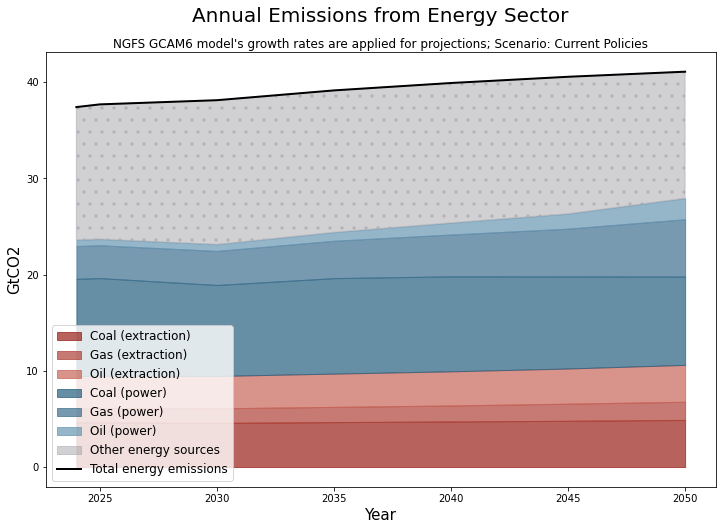
\includegraphics[width=\textwidth]{Figures/script 4.1 - current policy - annaul.png}
    \end{subfigure}
    \hfill
    \begin{subfigure}{0.48\textwidth}
        \centering
        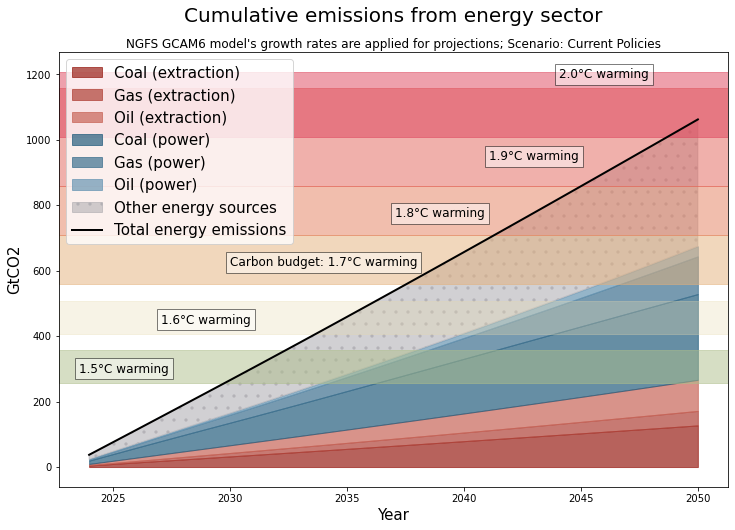
\includegraphics[width=\textwidth]{Figures/script 4.1 - current policy - cumulative.png}
    \end{subfigure}

    \vspace{1em}

    \begin{subfigure}{0.48\textwidth}
        \centering
        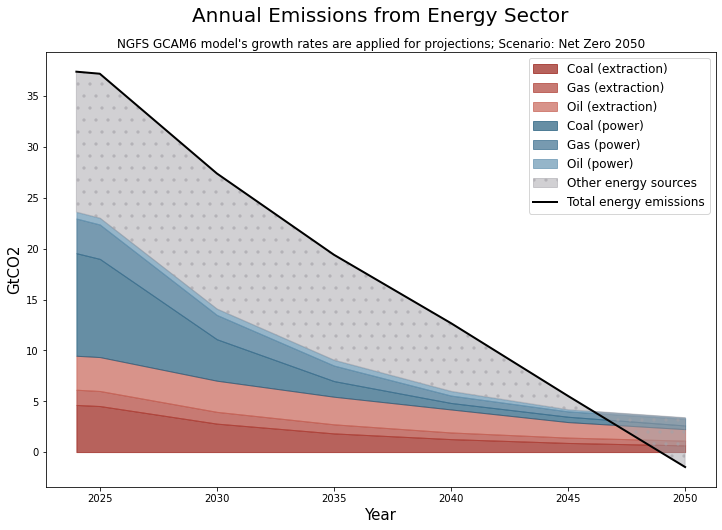
\includegraphics[width=\textwidth]{Figures/script 4.1 - netzero - annaul.png}
    \end{subfigure}
    \hfill
    \begin{subfigure}{0.48\textwidth}
        \centering
        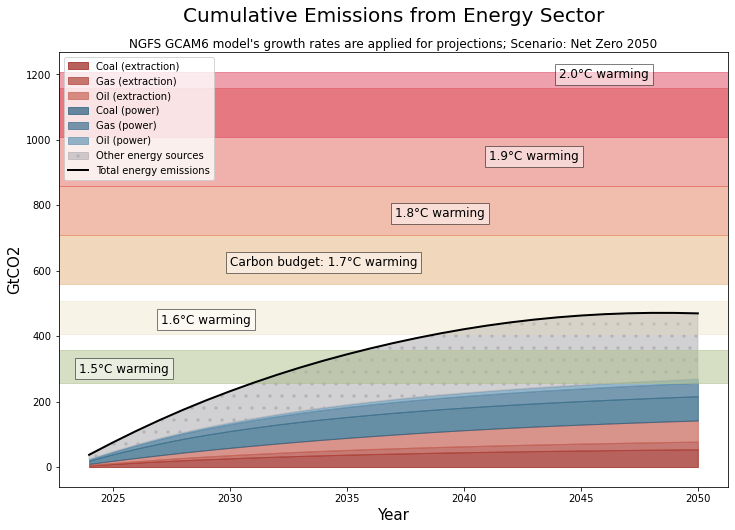
\includegraphics[width=\textwidth]{Figures/script 4.1 - netzero - cumulative.png}
    \end{subfigure}
    \caption{The annual (left) and cumulative (right) energy-related emissions under the NGFS GCAM6.0 current policy scenario (top) and net zero 2050 scenario (bottom) relative to the 50\%-67\% remaining carbon budgets (see Table~\ref{tab:RemainingCarbonBudgets}) for each tenth of a degree of global warming.}\label{fig:BAUNZScenarios}
\end{figure}

The question thus is how to make the NGFS net-zero 2050 scenario consistent with the remaining 1.5°C 50\% carbon budget, as 1.5°C is deemed by climate scientists to represent a physical limit beyond which several climate tipping points will likely be crossed and climate extremes will become much more severe. More generally, our method presented below enables one to make any net-zero scenario (e.g., from the IEA or IPCC) consistent with the remaining carbon budget for any chosen maximum degree of global warming (e.g., 1.6°C) with a certain probability (e.g., 67\%).\newline
\indent We observe from Table~\ref{tab:OvershootNGFS} that the NGFS net zero 2050 scenario overshoots the remaining carbon budget to limit global warming by at least 31\% (or more given the further depleted carbon budgets).\newline

\begin{table}[H]
    \centering
    \caption{Overshoot (if $>1$) of the cumulative 2025-2050 emissions under the NGFS Net Zero 2050 scenario relative to the remaining carbon budget associated with different temperatures (rows) and different probabilities (columns).}\label{tab:OvershootNGFS}
    \begin{tabular}{ccc}
        \hline
        Temperature Increase & Probability 50\% & Probability 67\% \\ \hline
        1.5°C & 1.31 & 1.82 \\ 
        1.6°C & 0.92 & 1.15 \\ 
        1.7°C & 0.66 & 0.84 \\ 
        1.8°C & 0.55 & 0.66 \\ 
        1.9°C & 0.41 & 0.55 \\ 
        2.0°C & 0.39 & 0.47 \\ \hline
    \end{tabular}
\end{table}


\noindent While there could be a number of various approaches to align total cumulative emissions with global remaining carbon budget, we choose to adjust all countries, all fossil fuel types (coal, oil, gas), at each time by same increased decarbonization rate $r>1$. This approach allows us to maintain relative country-$y$, fuel-$f$ and time-$t$ specific pathways originally modelled by by NGFS GCAM 6 model; thus retaining the richness of the original modeling framework.\newline
\indent In our algorithm to make the net zero 2050 scenario carbon budget consistent, we apply the following assumptions:

\begin{enumerate}
    \item The same reduction factor (\textit{r}) is applied to annual change rates for all fossil fuel types, in all countries, at each time of the decarbonization horizon.
    \item Annual change rates are capped at -100\% to ensure that no negative values occur. 
    \item In the original NGFS model, some countries can experience intermediary phase-out with later re-introduction of the fossil fuels back in their power or extraction sectors. We assume that in this edge case, the associated CO2 emissions of reintroducing fossil fuels are of the same level amount as the NGFS emission level amount $S^{s_{level},e}_{y,f,t}$ under scenario $s$ (see Section~\ref{ap:DataScenarioConstruction}), as you cannot divide by zero in equation~\ref{eq:EmissionReductionRelatives2} for $E_{y,f,t-1}^{s_2}=0$.
    \item Positive annual change rates are reduced by the same factor to maintain balance between countries reducing their fossil fuel emissions and those increasing them.
\end{enumerate}

\noindent We first pick a range of values for possible decarbonization rates $r>1$. Since the emission overshoot for the 1.5°C 50\% remaining carbon budget is 31\% (see Table~\ref{tab:OvershootNGFS}), a reasonable range and step size is:
\begin{align}
    r = 
    \begin{cases}
    r_{max} = 31\% * 10\\
    r_{min} = 31\% / 10\\
    \text{Step size} = 0.001
    \end{cases}
\end{align}
The relative emission reduction under net zero 2050 scenario $s_2$ is given by
\begin{equation}
     \ubar{\Delta} E^{s_2}_{y,f,\tau} = \frac{E^{s_2}_{y,f,\tau}-E^{s_2}_{y,f,\tau-1}}{E^{s_2}_{y,f,\tau-1}}= 
 \begin{cases}
   \in (0,-1], & \text{if}  E^{s_2}_{y,f,\tau}<E^{s_2}_{y,f,\tau-1}  \\
    \geq 1, & \text{if }  E^{s_2}_{y,f,\tau}\geq E^{s_2}_{y,f,\tau-1}, \label{eq:EmissionReductionRelatives2}
\end{cases}  
\end{equation}
for a $s_2$ scenario absent negative emissions (as the NGFS power sector net zero 2050 scenario applied to our data is).\footnote{We use $\ubar{\Delta} E$ to distinguish the relative emission reduction from the absolute emission reduction $\Delta E$.} Under the 1.5°C 50\% carbon budget consistent net zero scenario $s_3$, we update the relative emission reduction under net zero 2050 scenario $s_2$ to
\begin{equation}
    \ubar{\Delta} E^{s_{3}}_{y,f,\tau} =
    \begin{cases}
    \max( \ubar{\Delta} E^{s_{2}}_{y,f,\tau} * r, -1), & \text{if }    \ubar{\Delta} E^{s_{2}}_{y,f,\tau}  < 0 \\
    \frac{ \ubar{\Delta} E^{s_{2}}_{y,f,\tau}}{r}, & \text{if }   \ubar{\Delta} E^{s_{2}}_{y,f,\tau}  \geq 0.
\end{cases}
\end{equation}
To obtain the 1.5°C 50\% carbon budget consistent $s_3$ emission pathway $E^{s_3}_{y,f,t}$, for each $\tau \in (t,T]$, we iteratively apply $1+ \ubar{\Delta} E^{s_{3}}_{y,f,\tau}$ to the initial emissions $E^{data}_{y,f,t}$ as given by the Forward Analytics data for $t=2024$ (or IEA data for overall energy related emissions). To get the $E^{s_3}_{y,f,t+1}$ emission under the $s_3$ pathway, we do:
\begin{equation}
    E^{s_3}_{y,f,t+1} = E^{data}_{y,f,t} * \Pi_{\tau=t+1}^{t+1} (1+ \ubar{\Delta} E^{s_{3}}_{y,f,\tau})
\end{equation}
More generally to get the $\tau\in (t,T]$ emission under the $s_3$ pathway (e.g., $\tau=t+3$), we do:
\begin{equation}
    E^{s_3}_{y,f,\tau} = E^{data}_{y,f,t} * \Pi_{s=t+1}^\tau (1+ \ubar{\Delta} E^{s_{3}}_{y,f,s})
\end{equation}
Summing up the emissions over $[t=2024,T=2050]$ gives the cumulative emissions that the $s_3$ pathway generates:
\begin{equation}
    E^{s_3}_{y,f,t,T} = \sum_{\tau=t}^T E^{s_3}_{y,f,\tau}.
\end{equation}
The algorithm ends when there is a reduction factor $r$ that satisfies equation~\ref{eq:AlgorithmStop}, where cumulative total energy emissions are aligned with the carbon budget (CB) for limiting global warming to 1.5°C with 50\% likelihood within 1\% range (see Table~\ref{tab:RemainingCarbonBudgets}):
\begin{equation}
       CB - 1\% * CB \leq \sum_{y \in \mathcal{Y}} \sum_{f \in \mathcal{F}} E^{s_3}_{y,f,t,T} \leq CB + 1\% * CB .\label{eq:AlgorithmStop}
\end{equation}
We find $r=1.79$. As you can see from equation~\ref{eq:AlgorithmStop}, one can flexibly chose another carbon budget to align the scenario with, and indeed pick another $s_2$ scenario to start with (i.e., before making the carbon budget adjustment).\newline
\indent For the purposes of the above algorithm, we referred to the carbon-budget aligned scenario, adapted from scenario $s_2$, as $s_3$. However, in the remainder of the paper we will simply refer to this as scenario $s_2$.


\hspace{1cm}\newline \newline


\begin{figure}[H]
    \centering
    \begin{subfigure}{0.48\textwidth}
        \centering
\includegraphics[width=\textwidth]{Figures/script 4.2 - v1 - nz15 - 50 - annual.png}
    \end{subfigure}
    \hfill
    \begin{subfigure}{0.48\textwidth}
        \centering
\includegraphics[width=\textwidth]{Figures/script 4.2 - v2 - nz15 - 50.png}
    \end{subfigure}
     \caption{Annual (left plot) and cumulative (right plot) emissions under the ``1.5°C 50\% carbon budget consistent net zero" scenario.}
\end{figure}

\subsection{Business-As-Usual and Net-Zero Scenario Construction}\label{ap:DataScenarioConstruction}

In this subsection, we expand in more detail on how we construct the NGFS current policy scenario and net zero scenario for annual emissions shown in Figure~\ref{fig:BAUNZScenarios}. The emission values on the y-axis of the left plots of Figure~\ref{fig:BAUNZScenarios} are obtained from Forward Analytics, except for total energy-related emissions. The total power sector emissions of coal, oil, and gas plants, respectively, are obtained by summing plant-level emissions of that type across all plants of that type in the world.\footnote{Plant-level emissions are given by the formula: annual CO\textsubscript{2} (in million tonnes) = capacity * capacity factor * heat rate (in Btu per kWh) * emission factor (kg of CO\textsubscript{2} per TJ) * $9.2427 \times 10^{-12}$.} Similarly, total extraction emissions of coal, oil, and gas mines/fields are obtained by summing mine/field-level emissions of that type across all mines/fields of that type in the world. For total energy emissions at the start of 2024 (black line in Figure~\ref{fig:BAUNZScenarios}), we take the 2023 energy-related emission estimate of 37.2 Gt CO\textsubscript{2} from the IEA.\footnote{IEA CO\textsubscript{2} Emissions in 2023, Published March 2024 | Available at: \url{https://www.iea.org/reports/co2-emissions-in-2023/emissions-grew-in-2023-but-clean-energy-is-limiting-the-growth\#abstract}.} We use the plant and extraction-site specific emissions data (for each capturing scope I and scope II emissions) of Forward Analytics at $t_0=2024$ because the NGFS does not provide a granular breakdown of emissions beyond energy-related emissions and total emissions per country; and these are neither broken down by fuel type nor by plant/extraction site.\newline
\indent Taking the Forward Analytics emission data as a starting point, we then apply the NGFS projections under ``current policies" (for top left plot of Figure~\ref{fig:BAUNZScenarios}) or ``net-zero 2050" (for bottom left plot of Figure~\ref{fig:BAUNZScenarios}). As noted, the NGFS does not have projections at the country-level broken down by fossil fuel type and sector (power/extraction), but it does have projections of primary energy outputs (extraction) and secondary energy outputs (power) in EJ broken down by country and fossil fuel type. Hence, we can convert this to emission projections and apply these (as rate of change) to our initial emissions ($t_0=2024)$ from Forward Analytics data.\newline
\indent For the projections of extraction emissions (primary energy), we use the conversion rates in Table~\ref{tab:ConversionRates} to express NGFS projected EJ as projected extraction emissions $E^{s_{NGFS},e_{extraction}}_{y,f,\tau}$ under scenario $s$ (is business as usual or net zero) for country $y$ of fossil fuel extraction type $f$ and time $\tau$.

\begin{table}[h!]
    \centering
    \caption{Conversion of 1 EJ to CO\textsubscript{2} emissions}\label{tab:ConversionRates}
    \begin{tabular}{ccc}
        \hline
        Fuel type & Conversion from 1 EJ & Conversion to CO\textsubscript{2}  \\ \hline
        Coal & 37.6 million ton coal equivalent & 1764 kg CO\textsubscript{2} per ton \\
        Oil & 163.4 million barrels of oil equivalent & 0.43 ton CO\textsubscript{2} per barrel \\
        Gas & 27.9 billion cubic meters & 1.9 kg CO\textsubscript{2} per cubic meter \\ \hline
    \end{tabular}
\end{table}

The conversion rates in Table~\ref{tab:ConversionRates} are obtained as follows:

\begin{itemize}
    \item \textit{Coal}: 1 EJ is converted to 34.12 million tonne(s) of coal equivalent according to International Energy Agency's (IEA) converter\footnote{Available at: \url{https://www.iea.org/data-and-statistics/data-tools/unit-converter}}, and by a factor of 1.1 to short ton (based on which the conversion to CO\textsubscript{2} is based), giving 37.6 million ton coal equivalent. CO\textsubscript{2} coefficient is obtained from Energy Information Agency\footnote{Available at: \url{https://www.eia.gov/environment/emissions/co2_vol_mass.php}} (EIA).
    \item \textit{Oil:} conversion factors from BP's Statistical Review of World Energy to convert EJ to million barrels oil equivalent\footnote{Available at: \url{https://www.bp.com/content/dam/bp/business-sites/en/global/corporate/pdfs/energy-economics/statistical-review/bp-stats-review-2022-approximate-conversion-factors.pdf}}. Emissions factors are taken from U.S. Environmental Protection Agency's (EPA) Greenhouse Gas Equivalencies Calculator\footnote{Available at: \url{https://www.epa.gov/energy/greenhouse-gas-equivalencies-calculator-calculations-and-references}}.
    \item \textit{Gas:} similarly is converted to cubic meters using conversion factors from BP, and CO\textsubscript{2} coefficients are used from EIA.
\end{itemize}

To obtain the imputed NGFS projections of power sector emissions under the business as usual and net zero scenarios in~\ref{fig:BAUNZScenarios},we first use the factor 277,777,777 (or 277.8 TWh as reported by the IEA's conversion tool\footnotemark[3]) to convert EJ to MWh. Next, we obtain the projected power sector emissions by multiplying the NGFS secondary energy projection $S^{s_{level},e_{power}}_{y,f,\tau}$(expressed in MWh) for scenario $s$ (is business as usual or net zero) in country $y$ for fossil fuel $f$ and time $\tau$ with the emission intensity $I_{y,f}$ for that country $y$ and fossil fuel type $f$:
\begin{equation}
E^{s_{level},e_{power}}_{y,f,\tau} = I_{y,f} \times S^{s_{level},e_{power}}_{y,f,\tau}
\label{eq:PowerSectorEmissions}, \end{equation}
where the superscript $e_{power}$ indicates these are power sector emissions. We obtain the emission intensity for that country $y$ and fuel type $f$ as the weighted average (by activity in MWh) of the emission intensity of the power sector plants in that country and of that fuel type:
 \begin{equation}
            I_{y,f} =  \frac{\sum_{l \in \mathcal{L}_{y,f}} I_{y,f,l} \times A_{y,f,l}}{\sum_{l \in \mathcal{L}_{y,f}} A_{y,f,l}}
        \end{equation}
where  $I_{y,f,l}$ is the emission intensity (in MtCO2 per MWh) for power plant $l$ in country $y$ of fossil fuel type $f$ from Forward Analytics data, $A_{y,f,l}$ is the activity (in MWh) for power plant $l$ in country $y$ of fossil fuel type $f$ from Forward Analytics data, and $\mathcal{L}_{y,f}$ are the set of power plants in country $y$ of fossil fuel type $f$.\newline
\indent Since we rely on our granular asset level emission data for $t_0=2024$ from Forward Analytics, we do not use the in-emissions-expressed NGFS projections for energy-related, extraction and power-sector in absolute levels (i.e., $E^{s_{level},e_{energy-related}}_{y,\tau}$, $E^{s_{level},e_{extraction}}_{y,f,\tau}$, $E^{s_{level},e_{power}}_{y,f,\tau}$, respectively), but as relative changes as follows (for $t\in[t_0+1,T]$):x

\begin{align} \label{eq:EmissionProjections}
E^{s,e}_{y,l,t}&=
E^{e,data}_{y,l,t_0} \times \prod^{t}_{\tau=t_0+1} (1 + \frac{E^{s_{level}, e}_{y,\tau}-E^{s_{level}, e}_{y,\tau-1}}{E^{s_{level}, e}_{y,\tau-1}}) \\ \nonumber
&=E^{e,data}_{y,l,t_0} \times \prod^{t}_{\tau=t_0+1} \frac{E^{s_{level}, e}_{y,\tau}}{E^{s_{level}, e}_{y,\tau-1}}.
\end{align}

We observe in equation~\ref{eq:EmissionProjections}, that given the initial emission data $E^{e}_{y,l,t_0}$ for energy in general (IEA, 37.2Gt), extraction sites (Forward Analytics) and power plants (Forward Analytics) at the country level $y$ and plant level $l$ (where for energy related emissions as a whole the subscript $l$ does not apply), we can project emissions under the NGFS $s=s_1$ business as usual scenario or $s=s_2$ net-zero 2050 scenario by multiplying it iteratively with the relative difference of the NGFS emission projections at the absolute level $\frac{E^{s_{level},e}_{y,\tau}}{E^{s_{level},e}_{y,\tau-1}}$. We note that the emission projections at the absolute level are country $y$ and fossil fuel type $f$ and sector $e$ specific, but not plant specific. So all plants in a given country of a given fossil fuel type and sector (extraction/power) experience the same growth rates under $s=s_1$ is business as ususal and $s=s_2$ net-zero 2050.\newline
\indent The annual emissions at each year $t \in [t_0+1,T]$ per fossil fuel and sector in Figure~\ref{fig:BAUNZScenarios} are obtained by summing plant or extraction-specific emissions $E^{s,e}_{y,l,f,t}$ across plants and countries (i.e.,
$E^{s,e}_{f,t}=\sum_{y\in \mathcal{Y}} \sum_{l \in \mathcal{L}_y} E^{s,e}_{y,l,f,t}$).






\end{document}

